\begin{center}
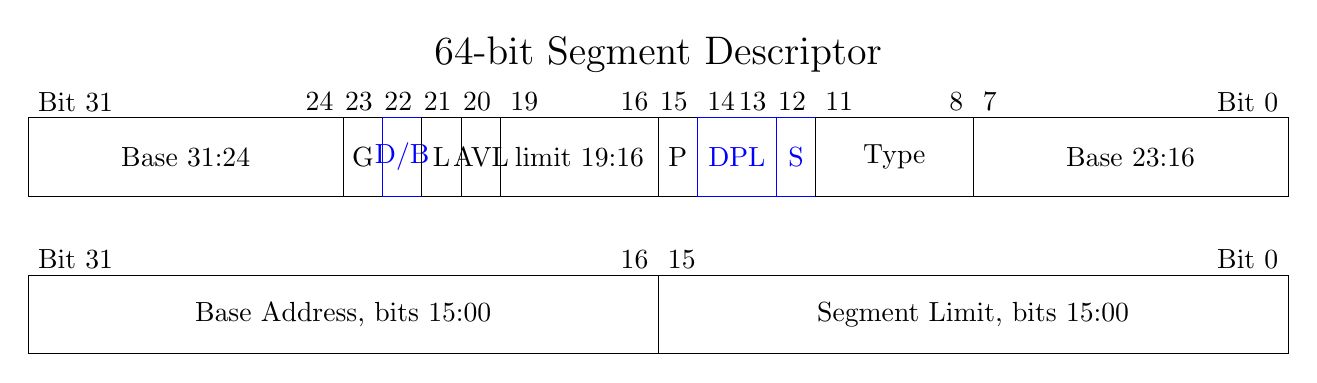
\begin{tikzpicture}
\draw node at (8,3.8) {{\Large 64-bit Segment Descriptor}};
\draw (0,2)  rectangle (4,3) node [pos=0.5] {Base 31:24}; \draw node at (0,3.2) [right] {Bit 31};
\draw (4,2)  rectangle (4.5,3) node [pos=0.5] {G}; \draw node at (4,3.2) [left] {24};
\draw [blue] (4.5,2)  rectangle (5,3) node [pos=0.5] {D/B};\draw node at (4.5,3.2) [left] {23};
\draw (5,2)  rectangle (5.5,3) node [pos=0.5] {L};\draw node at (5,3.2) [left] {22};
\draw (5.5,2)  rectangle (6,3) node [pos=0.5] {AVL}; \draw node at (5.5,3.2) [left] {21};
\draw (6,2)  rectangle (8,3) node [pos=0.5] {limit 19:16}; \draw node at (6,3.2) [left] {20}; \draw node at (6,3.2) [right] {19};
\draw (8,2)  rectangle (8.5,3) node [pos=0.5] {P}; \draw node at (8,3.2) [left] {16};
\draw [blue] (8.5,2)  rectangle (9.5,3) node [pos=0.5] {DPL};\draw node at (8.5,3.2) [left] {15}; \draw node at (8.5,3.2) [right] {14};
\draw [blue] (9.5,2) rectangle (10,3) node [pos=0.5] {S};\draw node at (9.5,3.2) [left] {13};
\draw (10,2)  rectangle (12,3) node [pos=0.5] {Type}; \draw node at (10,3.2) [left] {12}; \draw node at (10,3.2) [right] {11};
\draw (12,2)  rectangle (16,3) node [pos=0.5] {Base 23:16};\draw node at (12,3.2) [left] {8};
\draw (0,0)  rectangle (8,1) node [pos=0.5] {Base Address, bits 15:00};\draw node at (12,3.2) [right] {7};
\draw (8,0)  rectangle (16,1) node [pos=0.5] {Segment Limit, bits 15:00};
\draw node at (16,1.2) [left] {Bit 0};
\draw node at (8,1.2) [right] {15};
\draw node at (8,1.2) [left] {16};
\draw node at (0,1.2) [right] {Bit 31};
\draw node at (16,3.2) [left] {Bit 0};
\end{tikzpicture}

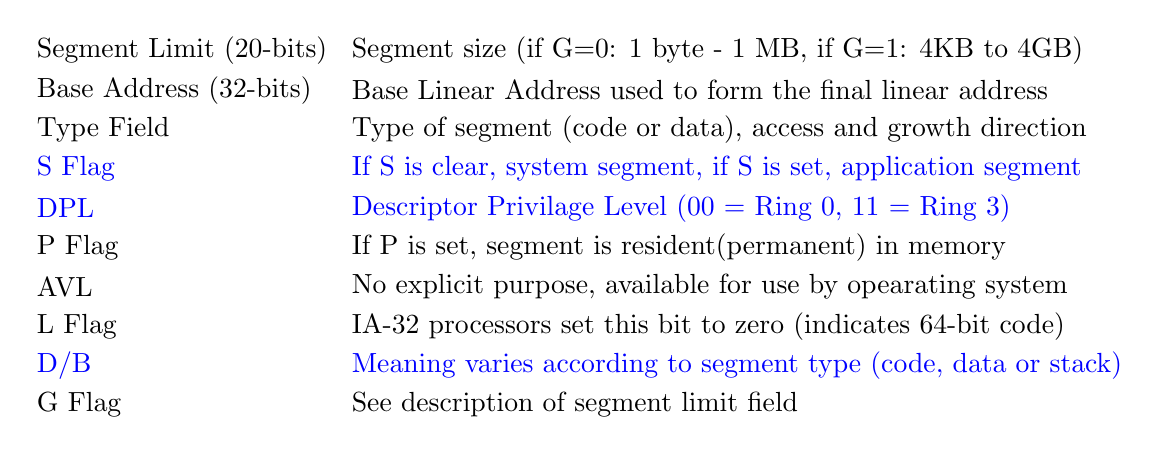
\begin{tikzpicture}
\draw node at (0,-0.5) [right] {Segment Limit (20-bits)};
\draw node at (0,-1) [right] {Base Address (32-bits)};
\draw node at (0,-1.5) [right] {Type Field};
\draw [blue] node at (0,-2) [right] {S Flag};
\draw [blue] node at (0,-2.5) [right] {DPL};
\draw node at (0,-3) [right] {P Flag};
\draw node at (0,-3.5) [right] {AVL};
\draw node at (0,-4) [right] {L Flag};
\draw [blue] node at (0,-4.5) [right] {D/B};
\draw node at (0,-5) [right] {G Flag};

\draw node at (4,-0.5) [right] {Segment size (if G=0: 1 byte - 1 MB, if G=1: 4KB to 4GB)};
\draw node at (4,-1) [right] {Base Linear Address used to form the final linear address};
\draw node at (4,-1.5) [right] {Type of segment (code or data), access and growth direction};
\draw [blue] node at (4,-2) [right] {If S is clear, system segment, if S is set, application segment};
\draw [blue] node at (4,-2.5) [right] {Descriptor Privilage Level (00 = Ring 0, 11 = Ring 3)};
\draw node at (4,-3) [right] {If P is set, segment is resident(permanent) in memory};
\draw node at (4,-3.5) [right] {No explicit purpose, available for use by opearating system};
\draw node at (4,-4) [right] {IA-32 processors set this bit to zero (indicates 64-bit code)};
\draw [blue] node at (4,-4.5) [right] {Meaning varies according to segment type (code, data or stack)};
\draw node at (4,-5) [right] {See description of segment limit field};
\end{tikzpicture}
\end{center}